\documentclass{article}
\usepackage{graphicx}
\usepackage[margin=1.5cm]{geometry}
\usepackage{csquotes}

\begin{document}

\title{Thursday Reading Assessment: Chapters 21-23 of \textit{Last Place on Earth}, Part I of Horizons}
\author{Prof. Jordan C. Hanson}

\maketitle

\section{Chapter 21 - Scott Sails On}

\begin{enumerate}
\item Robert Falcon Scott selected Manchurian ponies for his draught animals to help pull the sledges.  He elected to send a man named Cecil Meares in 1910 to Russia and Siberia to buy them, along with some dogs.  Describe the journey of Meares in this part of the world.  Where did he obtain the ponies?  What railroad did he have to use (it's rather famous)?  What was the condition of the ponies in the end? \\ \vspace{2cm}
\item Do you recall the story of the \textit{the broken pump}?  The Terra Nova is sailing through that dangerous part of the ocean between New Zealand and Antarctica.  The ship is equipped with a broken water pump.  What happened next?  How did the ship and crew survive? \\ \vspace{2cm}
\end{enumerate}

\section{Chapter 22 - The Base at Framheim}

\begin{enumerate}
\item
\begin{figure}[hb]
\centering
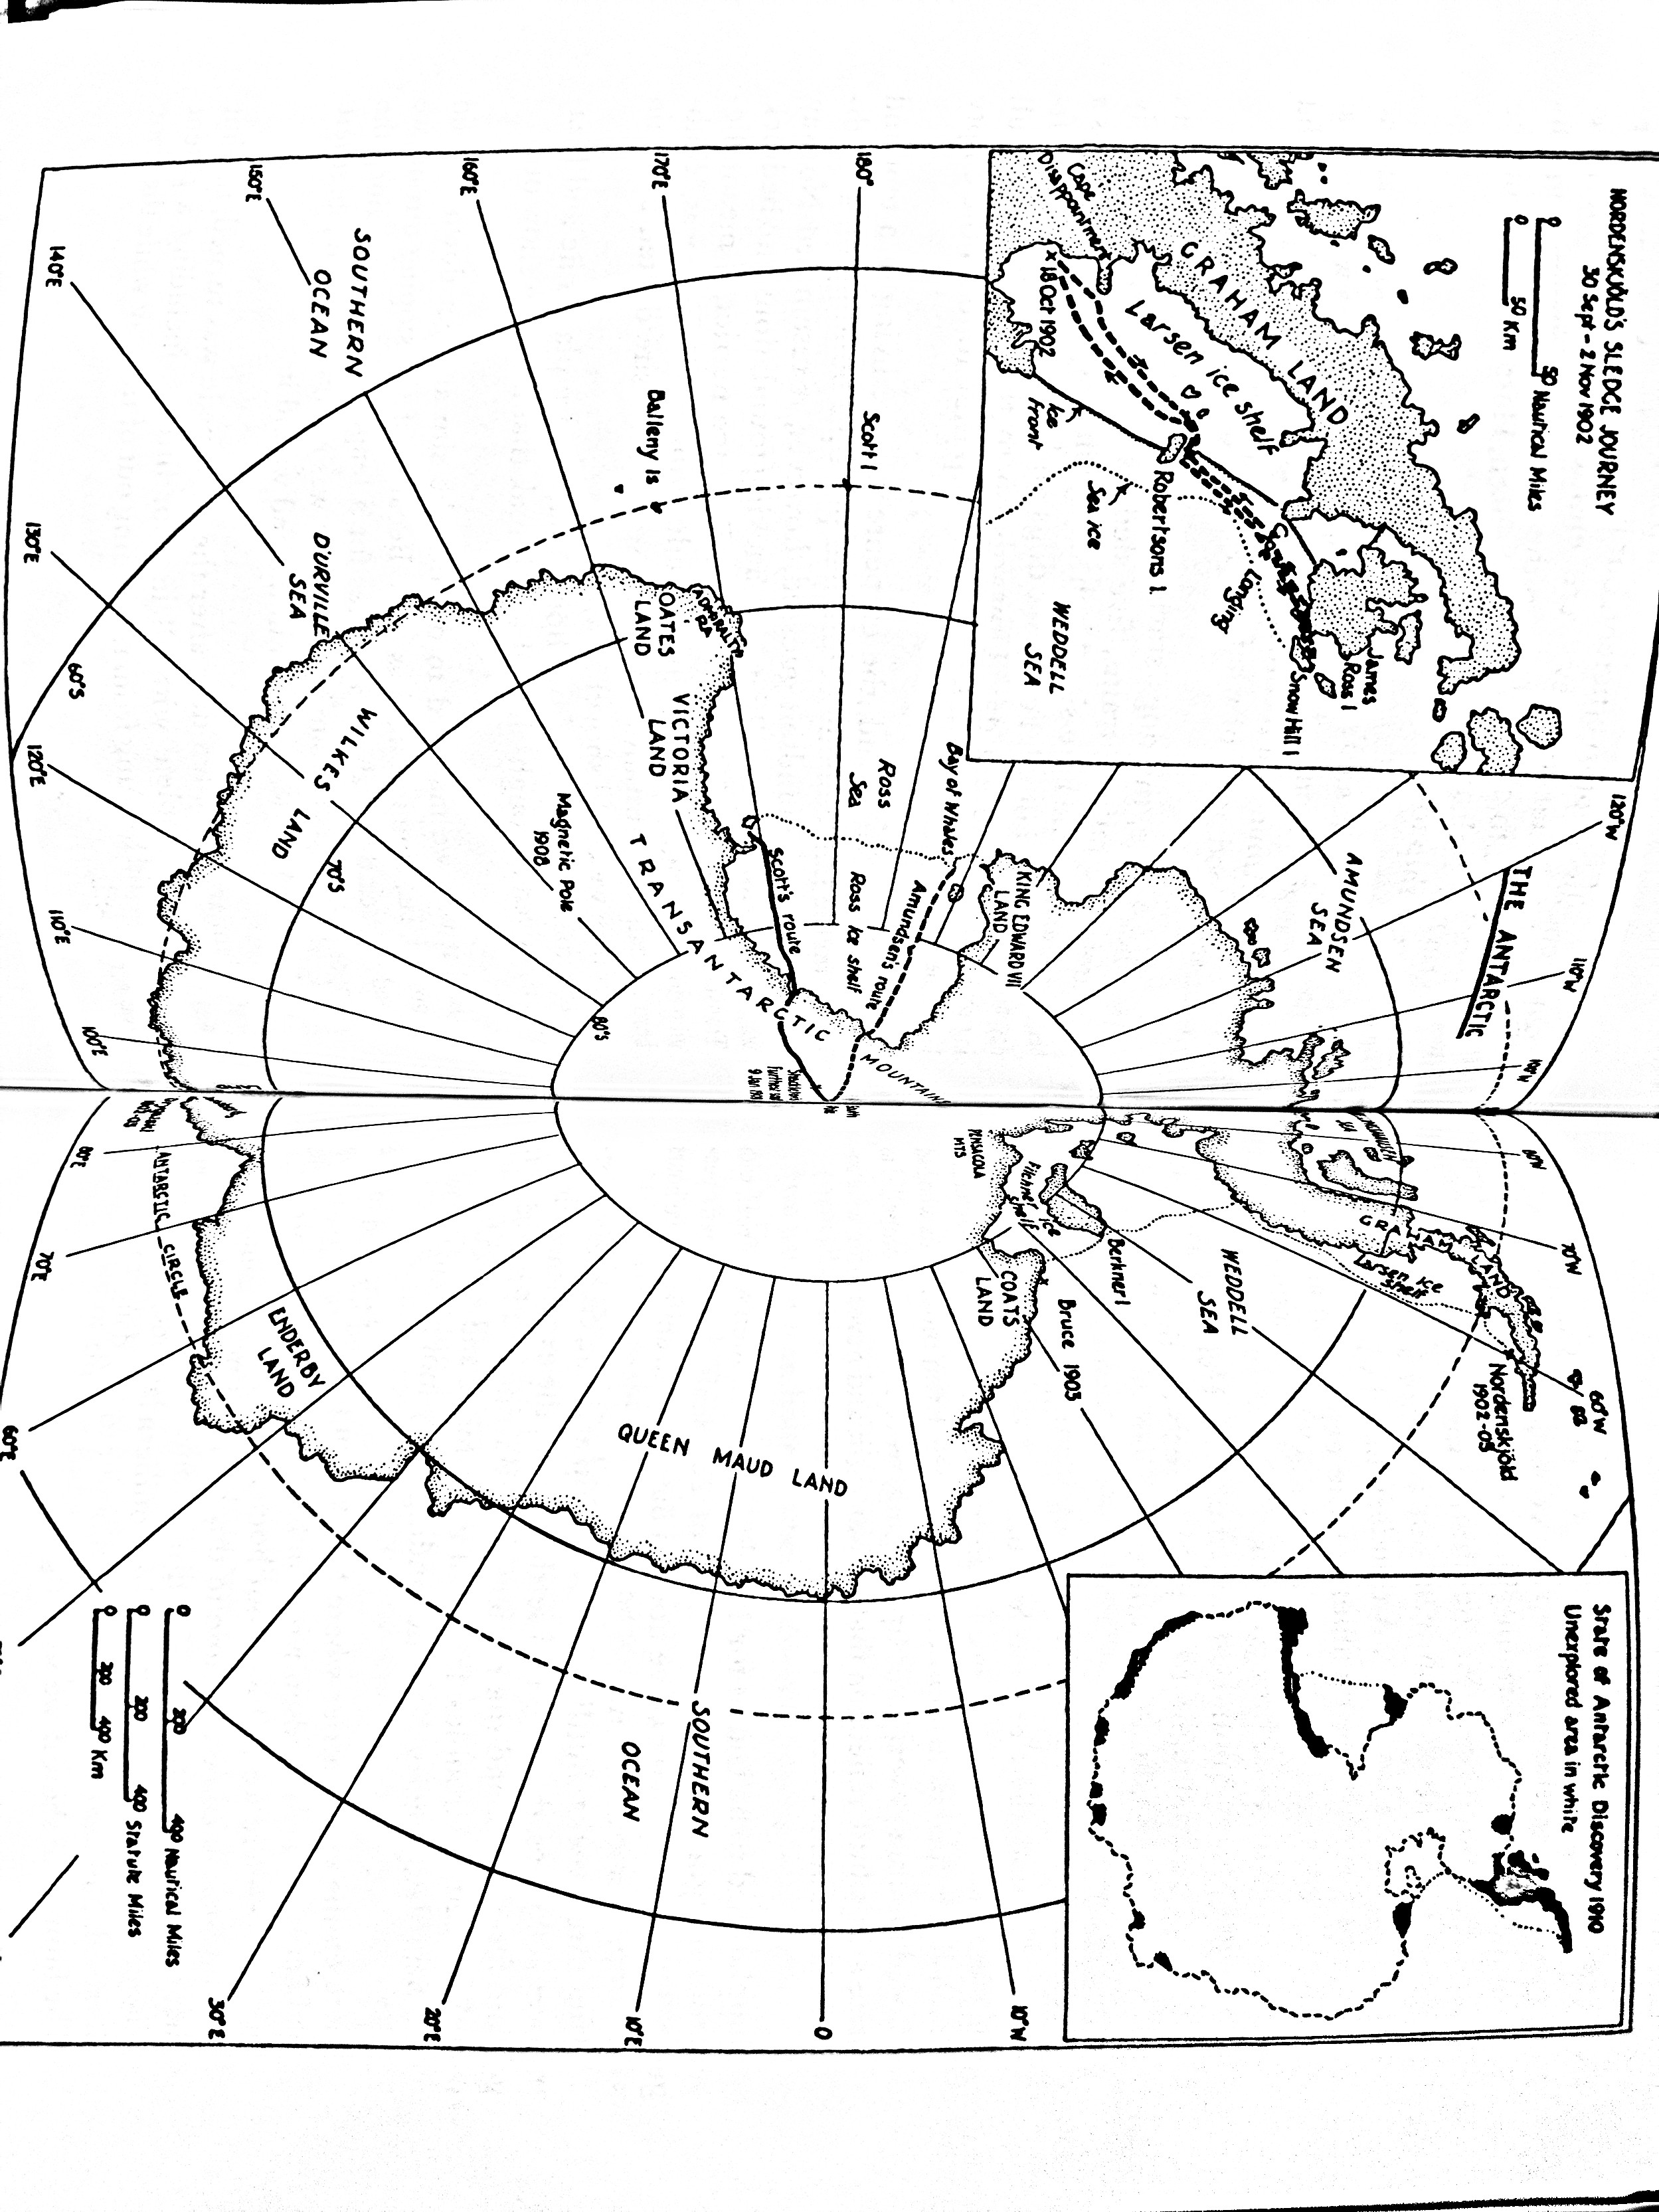
\includegraphics[width=0.3\textwidth,angle=90,trim=1cm 1cm 1cm 1cm,clip=true]{Map.jpg}
\caption{\label{fig:Map} A map from Ch. 21 showing the pathways of the two explorers to the South Pole.}
\end{figure}
In Fig. \ref{fig:Map}, we see the two landing points of the two South Pole seeking groups.  Do you see how they are choosing the closest landing points possible to South Pole?  Answer the following questions about the map.  a) Where is Scott landing?  b) Where is Amundsen landing?  c) Which proposed pathway is longer? d) How much of Antarctica had been explored at the time?
\item What were Amundsen's margins of safety?  For example, how much \textit{more} food did he place in his depots than the calculations suggested he needed? \\ \vspace{0.5cm}
\end{enumerate}

\section{Chapter 23 - Sledging with the Owner}
\begin{enumerate}
\item
\begin{figure}[hb]
\centering
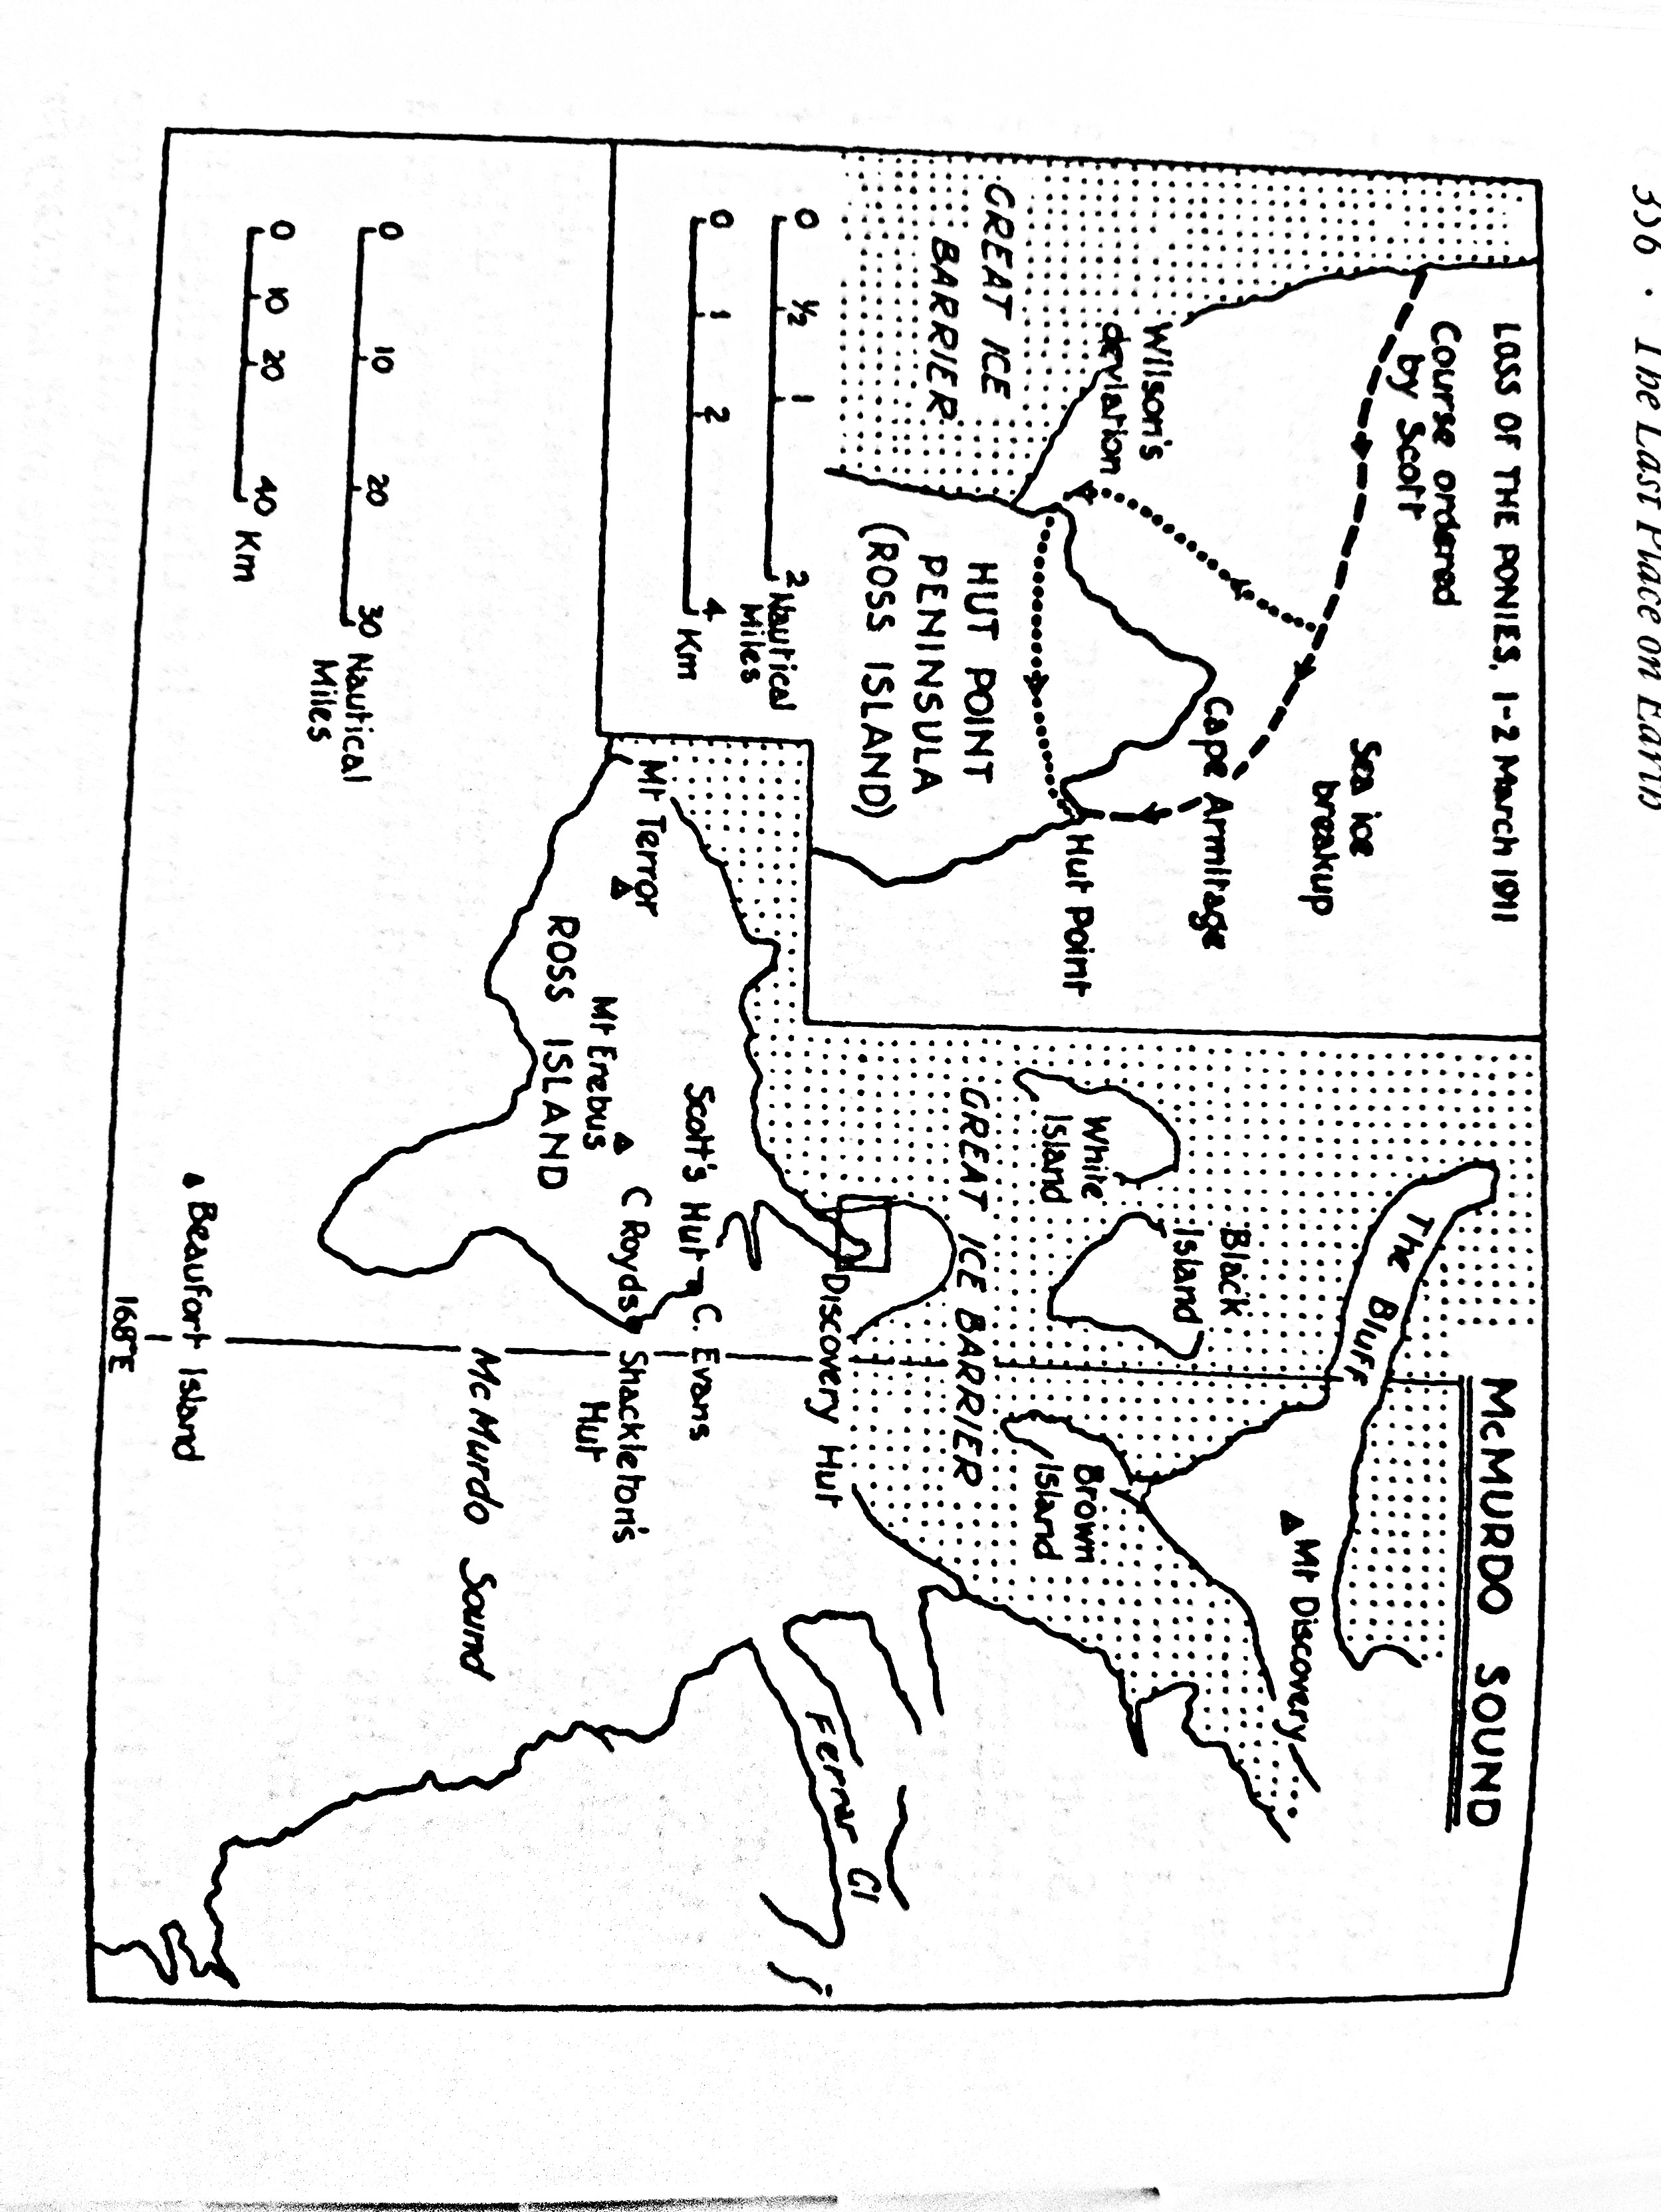
\includegraphics[width=0.3\textwidth,angle=90,trim=1cm 1cm 1cm 1cm,clip=true]{Map2.jpg}
\caption{\label{fig:Map2} A map from Ch. 22 showing the initial depot trip of Scott with the ponies.}
\end{figure}
In Fig. \ref{fig:Map2}, we see the journey back from the One Ton Depot of Scott's party.  a) What was the purpose of this journey?  b) What happened to the dogs versus the ponies?  How did each fare in the climate, and why?  c) Why did the men split off and go a different direction (upper left part of the map) instead of the way that Scott ordered?
\end{enumerate}

\section{Horizons - Part I}

\begin{enumerate}
\item
\begin{figure}[hb]
\centering
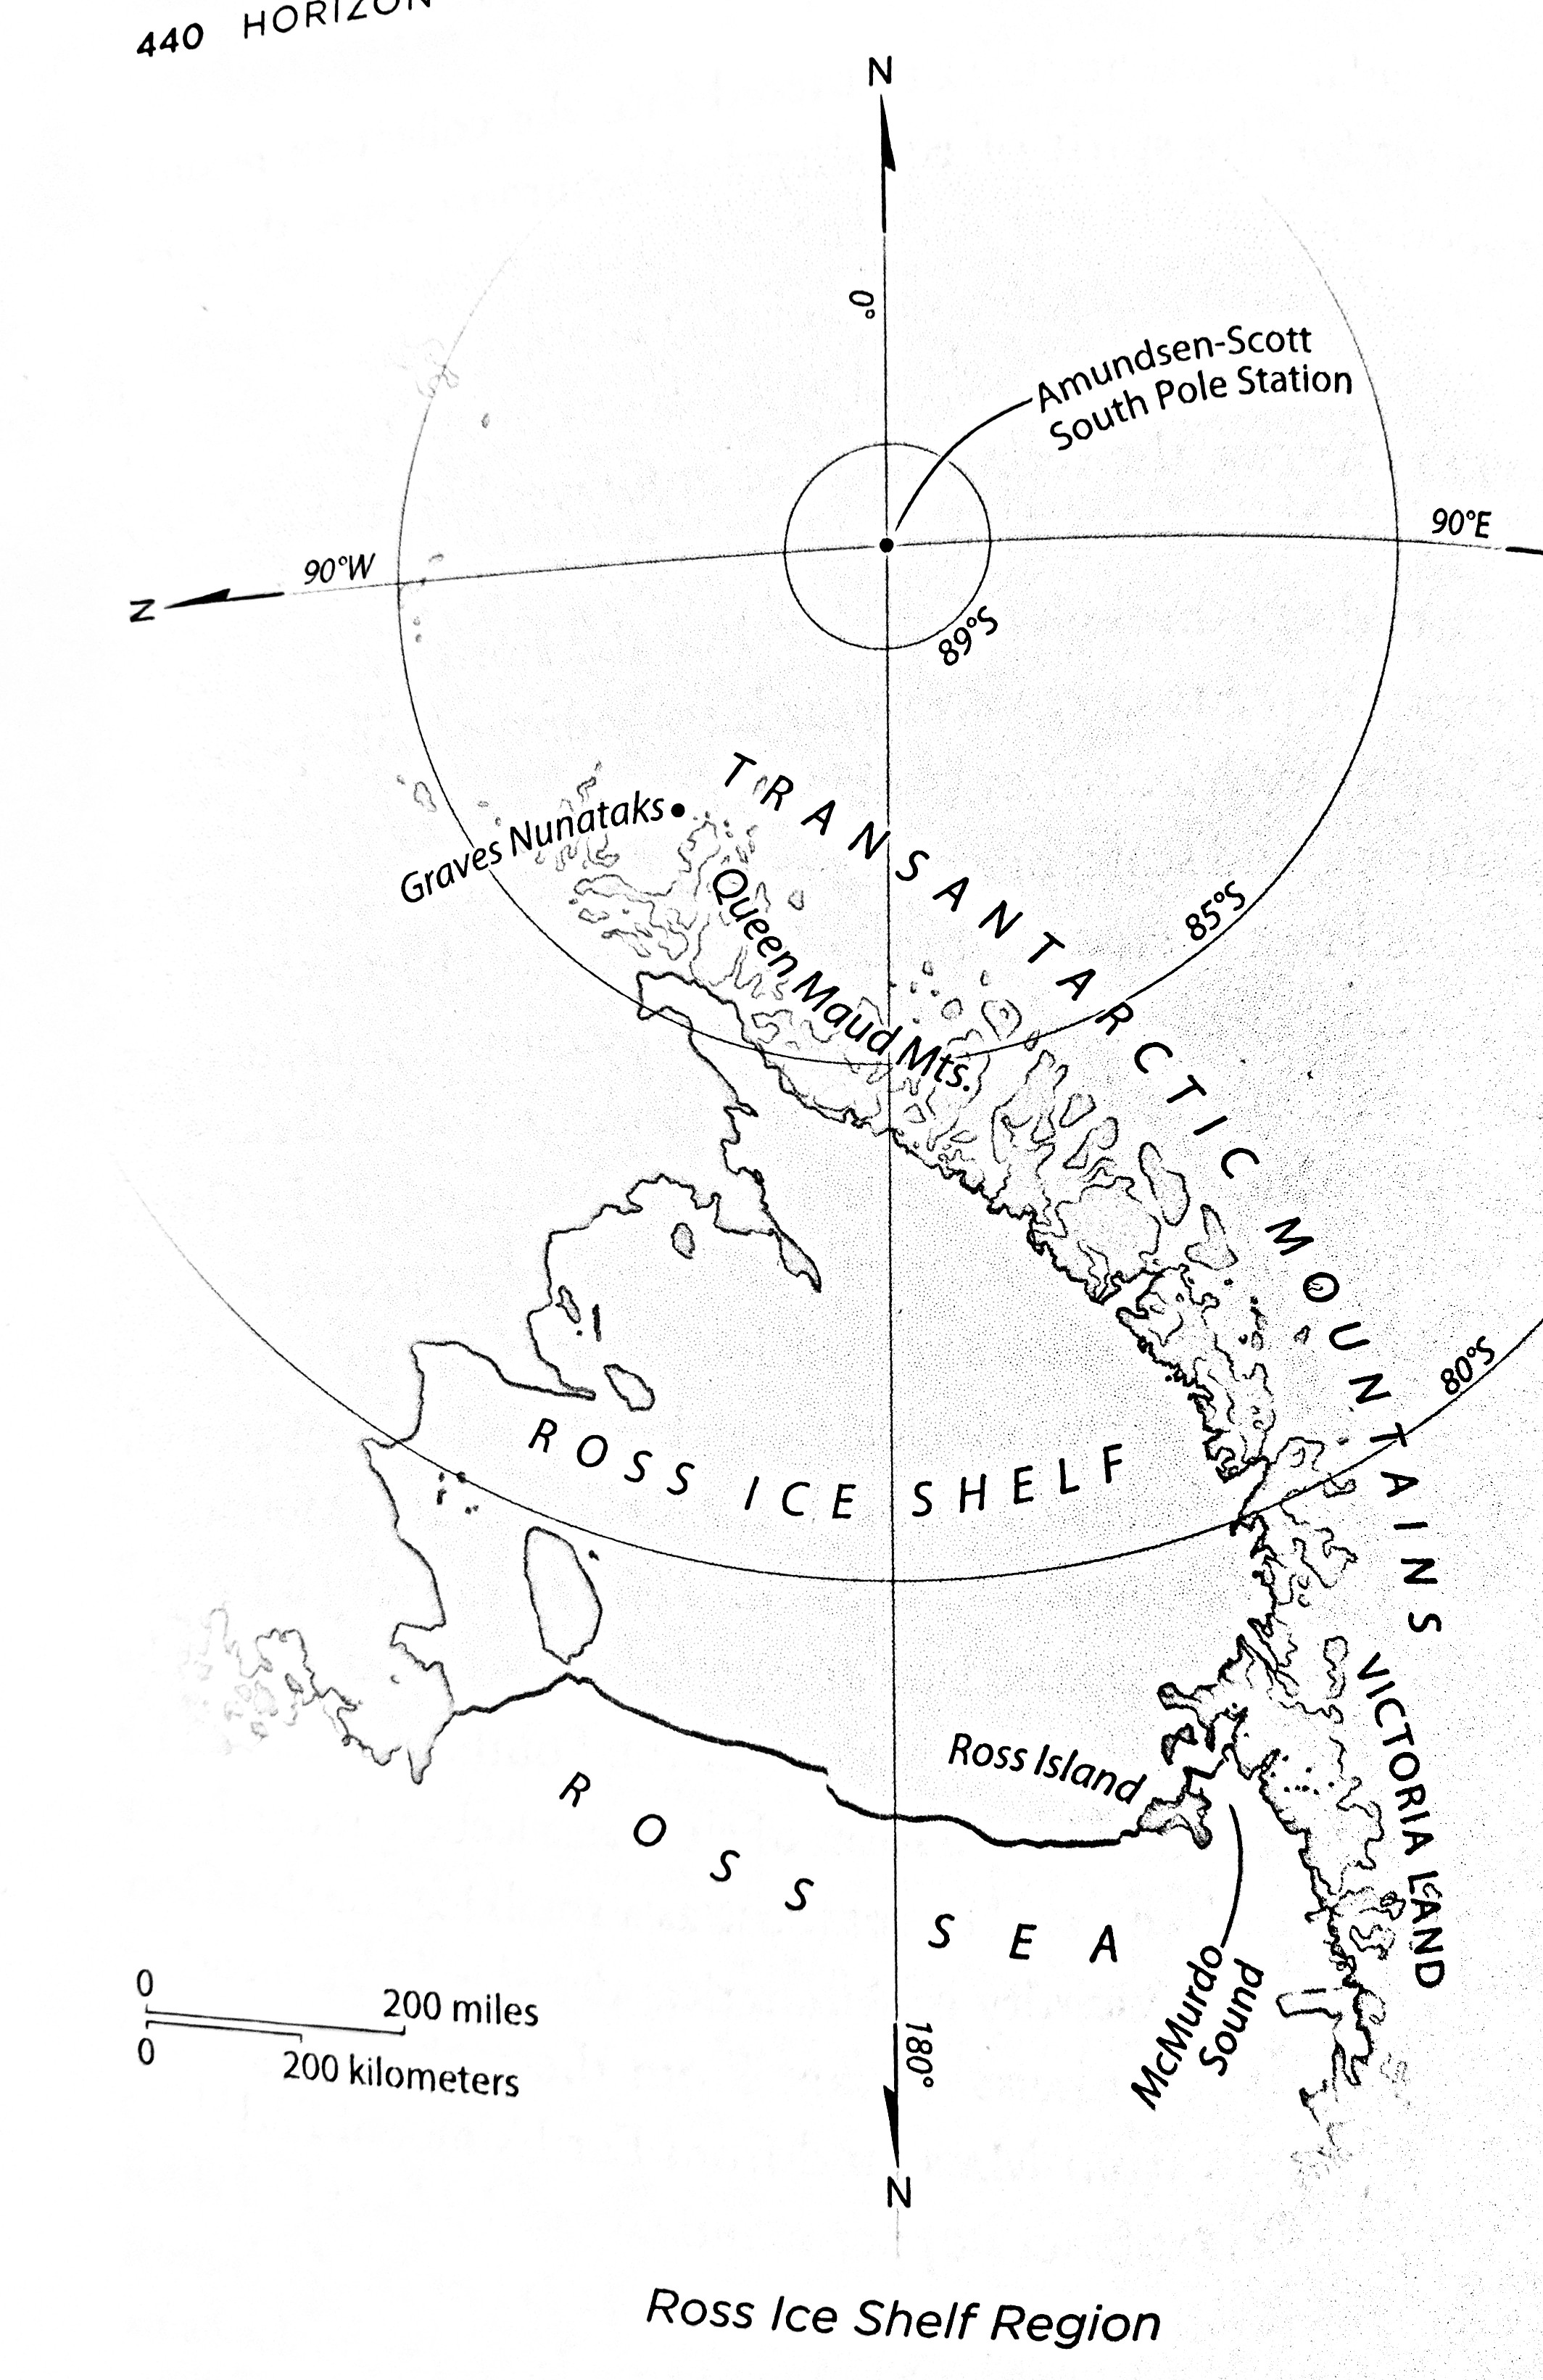
\includegraphics[width=0.33\textwidth,angle=0,trim=1cm 1cm 1cm 1cm,clip=true]{Map3.jpg}
\caption{\label{fig:Map3} A map from Ch. 22 showing the initial depot trip of Scott with the ponies.}
\end{figure}
Where in Fig. \ref{fig:Map3} is the author deployed?  For what are they searching, and why is it easy to find them there?  What are some of the author's observations about life in Antarctica?
\end{enumerate}

\end{document}
